\documentclass[../defence.tex]{subfiles}
\begin{document}

  \begin{frame}{Annormaler ganzzahliger Quanten Hall Effekt (QHE) in Graphen II}
    \begin{columns}[onlytextwidth, T]
      \column{\dimexpr\linewidth / 2}
        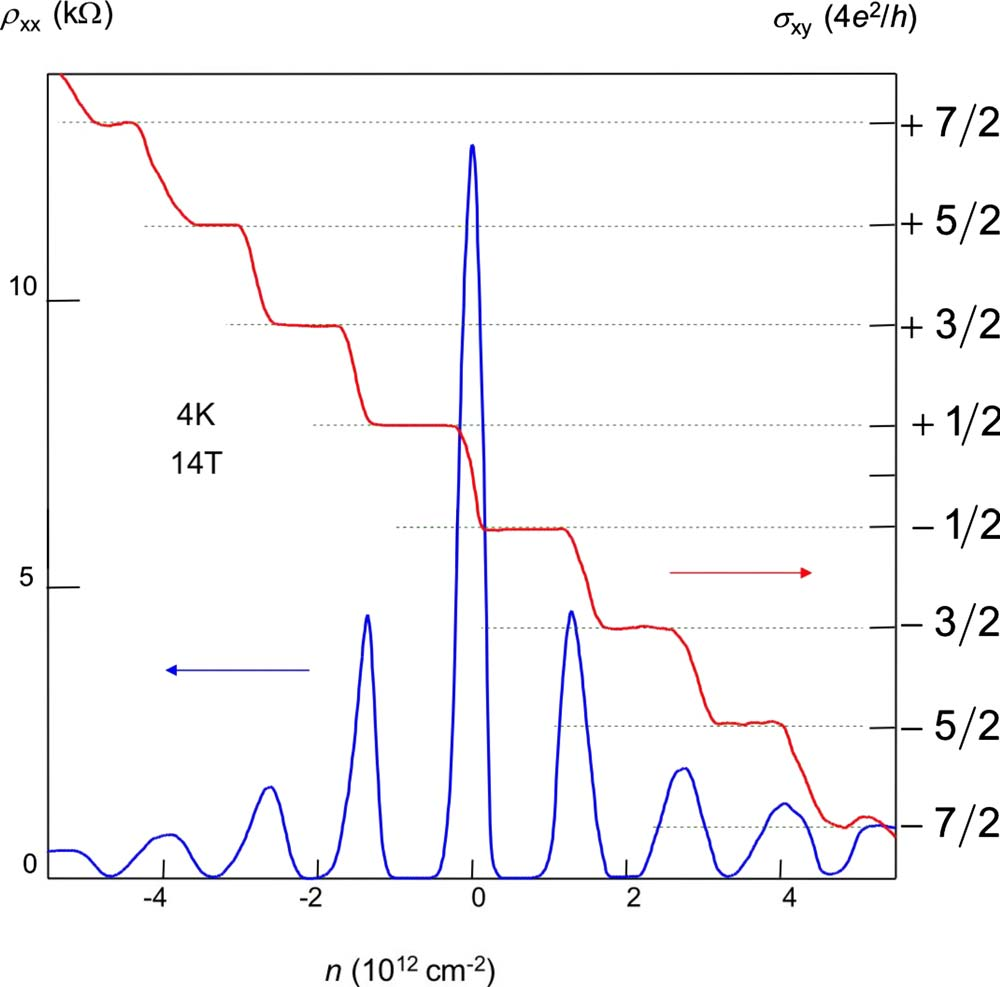
\includegraphics[width=\linewidth]{images/qhe.png}
        \cite{geim2007}
    \end{columns}
    \note{
    \begin{itemize}
      \item In blau: Longitudinalkomponente des Wiederstands
      \item In rot: Hall-Komponente der Leitfähigkeit $\rightarrow$ Kein Hall-Plateau bei $n=0$
    \end{itemize}
    }
  \end{frame}

\end{document}
